\documentclass{uebblatt}

\begin{document}

\section*{Guide zu Übungsblatt 8}

Tipp zu \textbf{Aufgabe 2a)}: Wenn~$V$ ein endlich-dimensionaler Vektorraum ist,
so ist~$V$ als Objekt der symmetrischen monoidalen Kategorie der Vektorräume
(mit dem gewöhnlichen Tensorprodukt als monoidale Struktur) dualisierbar
mit~$V^\vee = \Hom_k(V,k)$,~$\varepsilon(\vartheta \otimes v) =
\vartheta(v)$ und~$\eta(1) = \sum_i v_i \otimes \vartheta_i$ (wobei~$(v_i)_i$
eine Basis von~$V$ und~$(\vartheta_i)_i$ die zugehörige Dualbasis ist).

Bei \textbf{Aufgabe 2b)} sollte man keinesfalls einen gleichungsbasierten
Beweis führen! Mit den vielen Kohärenzisomorphismen kommt man dabei in Teufels
Küche. Führe deinen Beweis mit der grafischen Notation. Verwende folgende
Bausteine (die aus einem Artikel entnommen sind, den ich jetzt noch nicht
angebe):

\begin{center}
  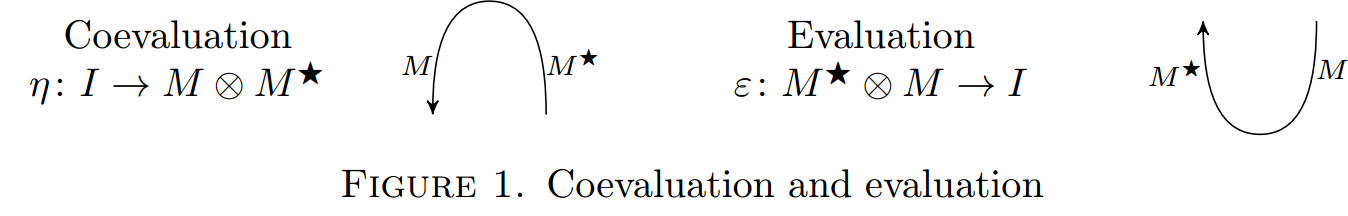
\includegraphics[scale=0.3]{images/ponto-shulman-1}

  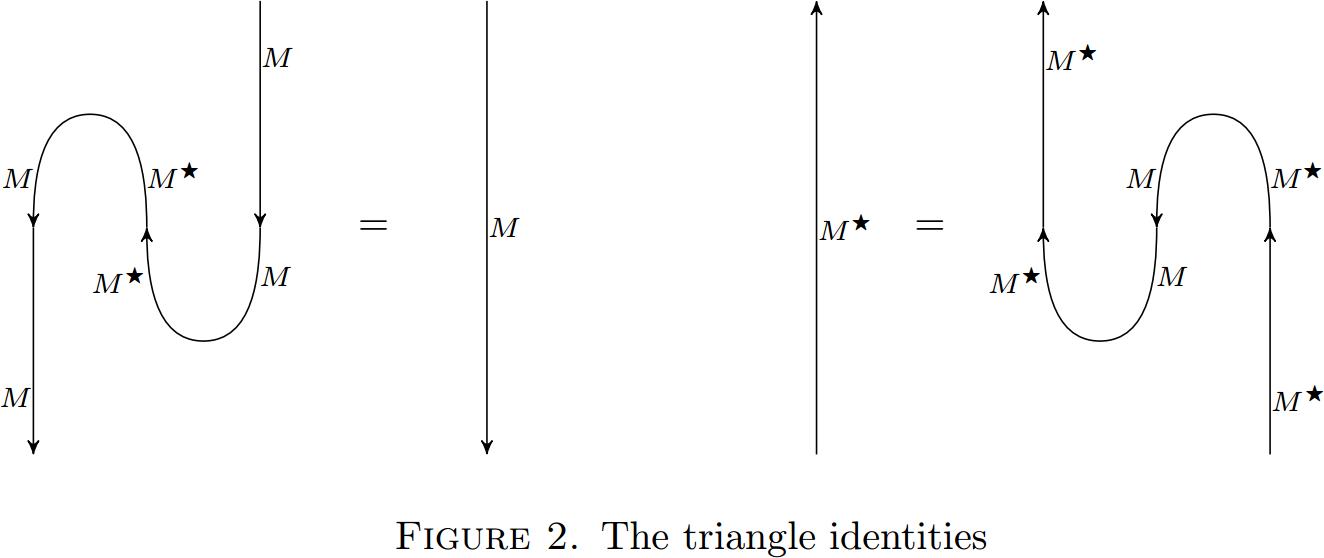
\includegraphics[scale=0.3]{images/ponto-shulman-2}

  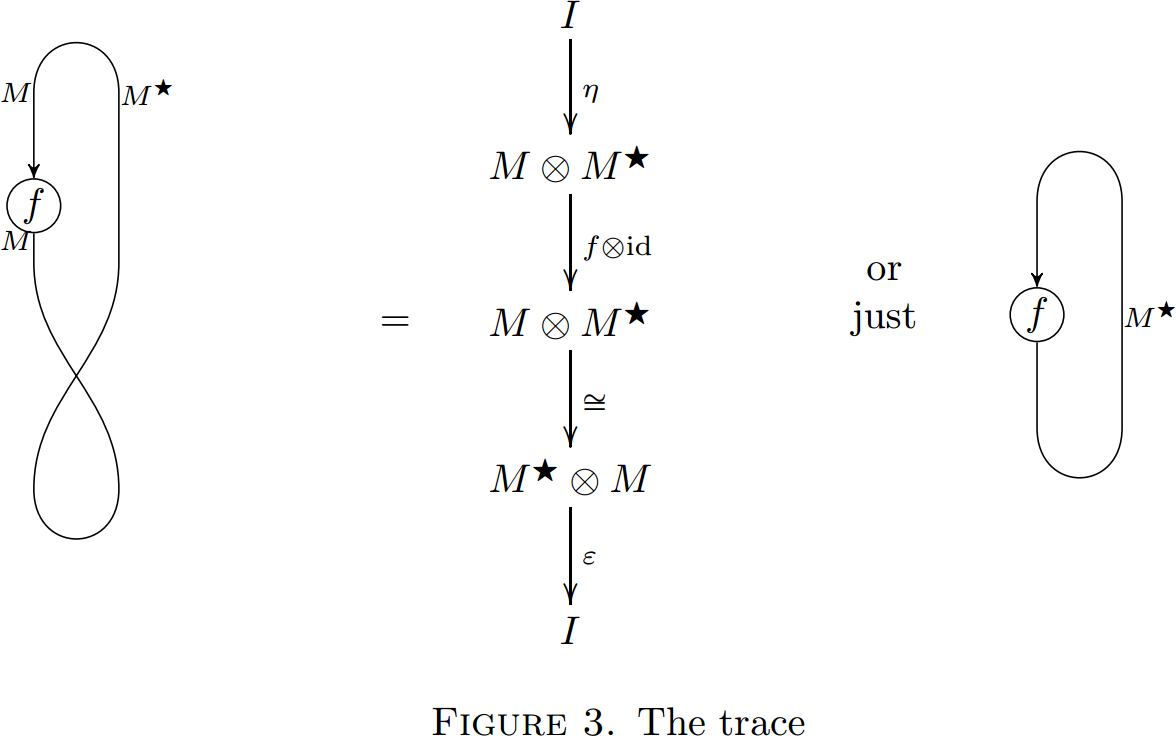
\includegraphics[scale=0.3]{images/ponto-shulman-3}
\end{center}

Um die Begriffe in \textbf{Aufgabe 2c)} zu klären, hilft vielleicht folgende
Skizze (vom Wikipedia-Eintrag zu Kobordismen). Sie illustriert einen Morphismus
von~$S^1$ nach~$S^1 \amalg S^1$.
\begin{center}
  
\includegraphics{images/pair-of-pants}
\end{center}

Bei \textbf{Aufgabe 3} soll man sich überlegen, wie diese Definitionen
sinnvollerweise auszusehen haben. Welche Isomorphismen sollte man fordern?
Welche Gleichheiten zwischen Morphismen?

\end{document}
